\section{Software Architecture}
\label{sec:sa}

本组源码分析涉及到的软件体系结构有:OO、Decorator、Adapter、Pipe、Logging、Interpreter、Layer

主要体系风格为:OBJECT ORIENTED和 DECORATOR \& ADAPTER

OBJECT ORIENTED三大主要特性:
封装:将不需要对外提供的内容都隐藏起来;把属性都隐藏,提供公共方法对其访问
继承:继承是一种联结类的层次模型,并且允许和鼓励类的重用,它提供了一种明确表述共性的方法。
多态:父类型的引用可以指向子类的对象。

所有outputstream的子类可以Upcast向上转型为outputstream作为参数输入。
\begin{figure}[h]
\centering
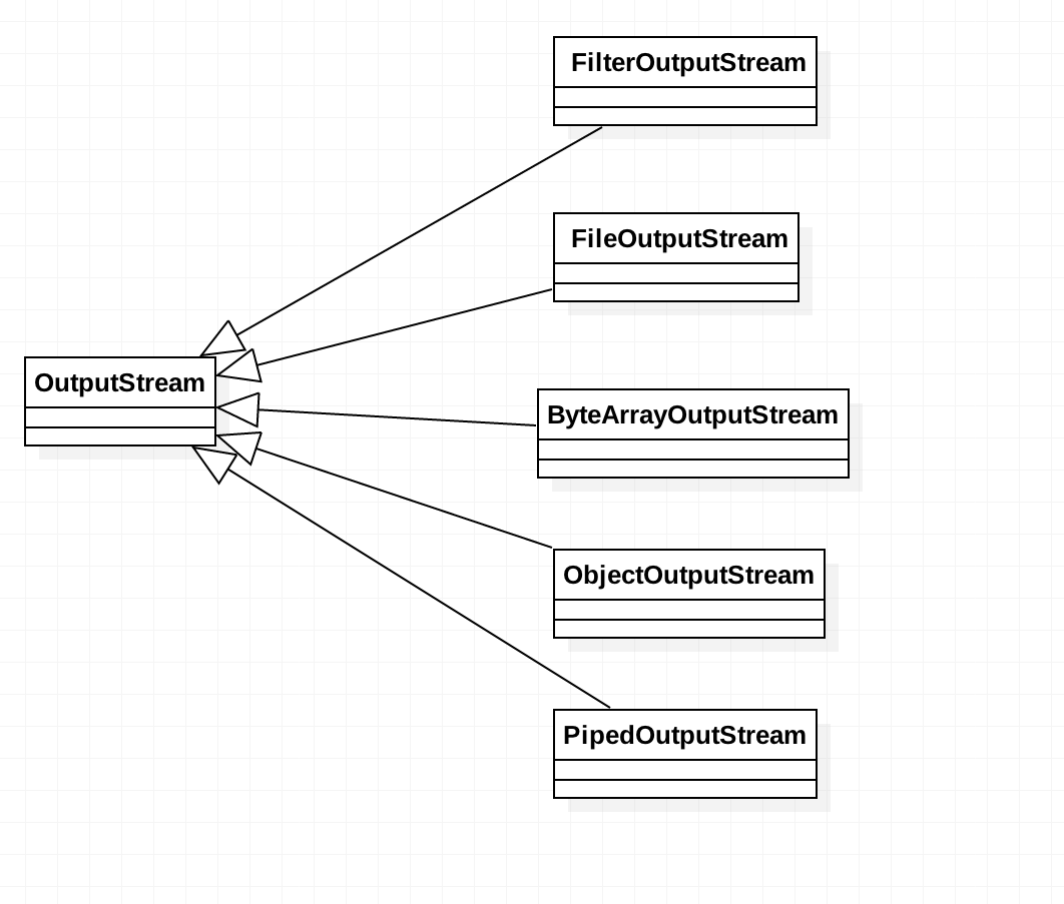
\includegraphics[width =1\linewidth]{output.png}
\caption{outputstream 及其子类}
\label{fig:OutputStream}
\end{figure}
begin{java}
public PositionCache(OutputStream out,
                     FileSystem.Statistics stats,
                     long pos) throws IOException {
  super(out);
  statistics = stats;
  position = pos;
}
end{java}
这里体现了面向对象体系结构风格中的多态性,任何outputStream的子类都可以Upcast,向上转型为outputstream,并作为参数输入
DECORATOR \& ADAPTER:
Decorator 装饰器 :对客户端透明的方式扩展对象的功能,是继承关系的一个替代方案,提供比继承更多的灵活性。使用原来被装饰的类的一个子类的实例,把客户端的调用委派到被装饰类。
Adapter适配器 :把一个类的接口变换成客户端所期待的另一种接口,从而使原本因接口原因不匹配而无法一起工作的两个类能够一起工作。适配类可以根据参数返还一个合适的实例给客户端。
总而言之:多态:父类型的引用可以指向子类的对象。
\begin{figure}[h]
\centering
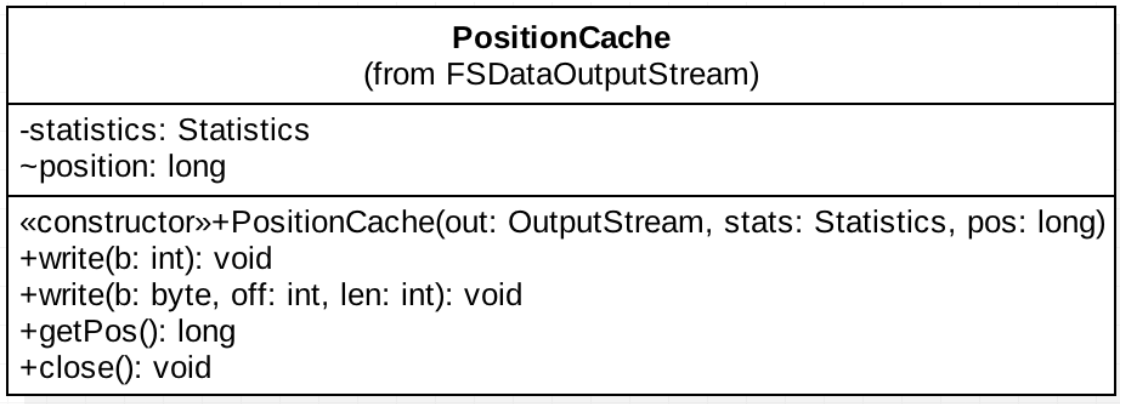
\includegraphics[width =1\linewidth]{positioncache.png}
\caption{PositionCache}
\label{fig:PositionCache}
\end{figure}
这里体现了装饰器这一体系风格,它对DataOutputStream的核心功能进行了拓展,添加了存储文件指针position的功能
和statistics属性
begin{java}
public void write(int b) throws IOException {
  out.write(b);
  position++;
  if (statistics != null) {
    statistics.incrementBytesWritten(1);
  }
}

public void write(byte b[], int off, int len) throws IOException {
  out.write(b, off, len);
  position += len;                            // update position
  if (statistics != null) {
    statistics.incrementBytesWritten(len);
  }
}
end{java}
这里体现了软件体系风格中适配器这一模式,在PositionCache这一子类中调用了outputstream中的write和close()方法。


%% 结束
\endinput
